 \chapter{Nevrologiske sykdommer}
		\section{Hva du skal ta med deg videre:}
			\begin{itemize}
				\item Husk FAST -Fjes -Arm -Språk -Tid.\\
				\item Ta et blodsukker.\\
				\item Drypp er en av de største risikofaktorene for slag.\\
				\item Slagpasienter som sliter språklig er ikke dumme.\\
				\item Regelmessig puls?\\
			\end{itemize}
		\section{Kort om denne delen...}
			Hjernen er hoveddelen av sentralnervesystemet. Det er ikke meningen å snakke om hele nervesystemet, men denne delen omhandler slag, drypp og demens som er noen av de største utfordringene vi har i dag. Jeg kommer ikke til å bruke mye pass på parkinsons og andre sykdommer da dette ville blitt for omfattende for dette dagsseminaret.
		\section{Anatomi}
			\paragraph{Et komplekst bilde}
				\begin{figure}[ht]
                      \centering
                      	\frame{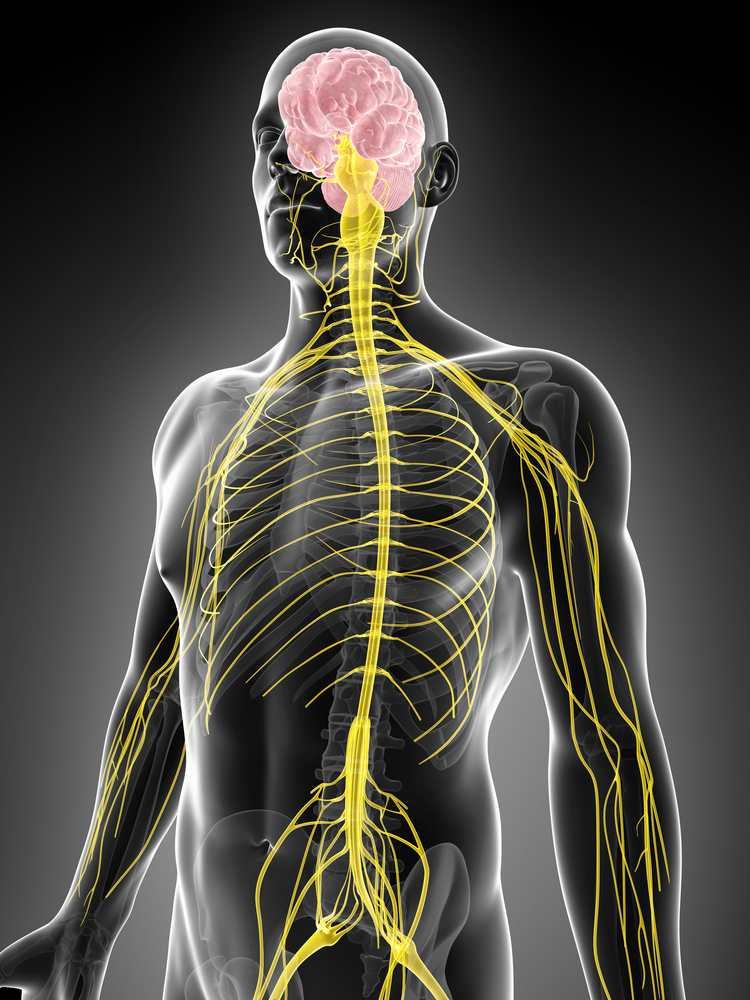
\includegraphics[width=3in]{./kap/bilder/nevro1.jpg}}%!!! må byttes ut, copyright Greys anatomy
                      \caption{Oversiktsbilde over det sentrale nervesystem}
                      %{Her ser vi et bilde som illusterer lungene og den antomiske oppbygningen}%\textit{tjenestetilbudene}.]
                    \end{figure}
			\paragraph{Inndelingen\\}
				Hjernen er forbundet med ryggmargen i medulla oblongata, eller den forlengede ryggmargen på norsk. Selve ryggmargen går omlag 2/3 ned av hele lengden av ryggen. 
		\section{Fysiologi}
			\paragraph{Kompleks struktur\\}
				Hjernen er organisert i områder som jobber med hver sine oppgaver. For eksempel sitter personligheten foran, rett bak pannen. Alle nervecellene er koblet sammen som et stort nettverk som løser hver sine oppgaver, men også jobber på kryss og tvers. 
			\paragraph{Plastisitet\\}
				En viktig egenskap er kalt "Hjernens plastisitet". Det betyr at hjernen kan reparere og til dels få tilbake tapte funksjoner igjen. for eksempel kan en person som har hatt slag trene seg opp ved å bruke en annen del av hjernen enn den som ble skadet. Det betyr også at selv om hjernen har områder som er spesialisert, kan disse områdene endre seg.
		\section{Patologi}
			\paragraph{Sykdommer i blodårene\\}
				Som beskrevet i \nameref{sec:athero} på side \pageref{sec:athero} %!!!
				er årsaken til slag og drypp en forkalking av blodårene og en plutselig redusert blodgjennomstrømning\cite{FA-athero}. Det som følger er omtrent som ved hjerteinfarkt: en del av hjernen mister oksygentilførselen, og nervene dør der blodsirkulasjonen stopper. Ettersom hvor den tette åren sitter blir symptomene lokalisert på kroppen.
					\begin{figure}[ht]
                      \centering
                      	\frame{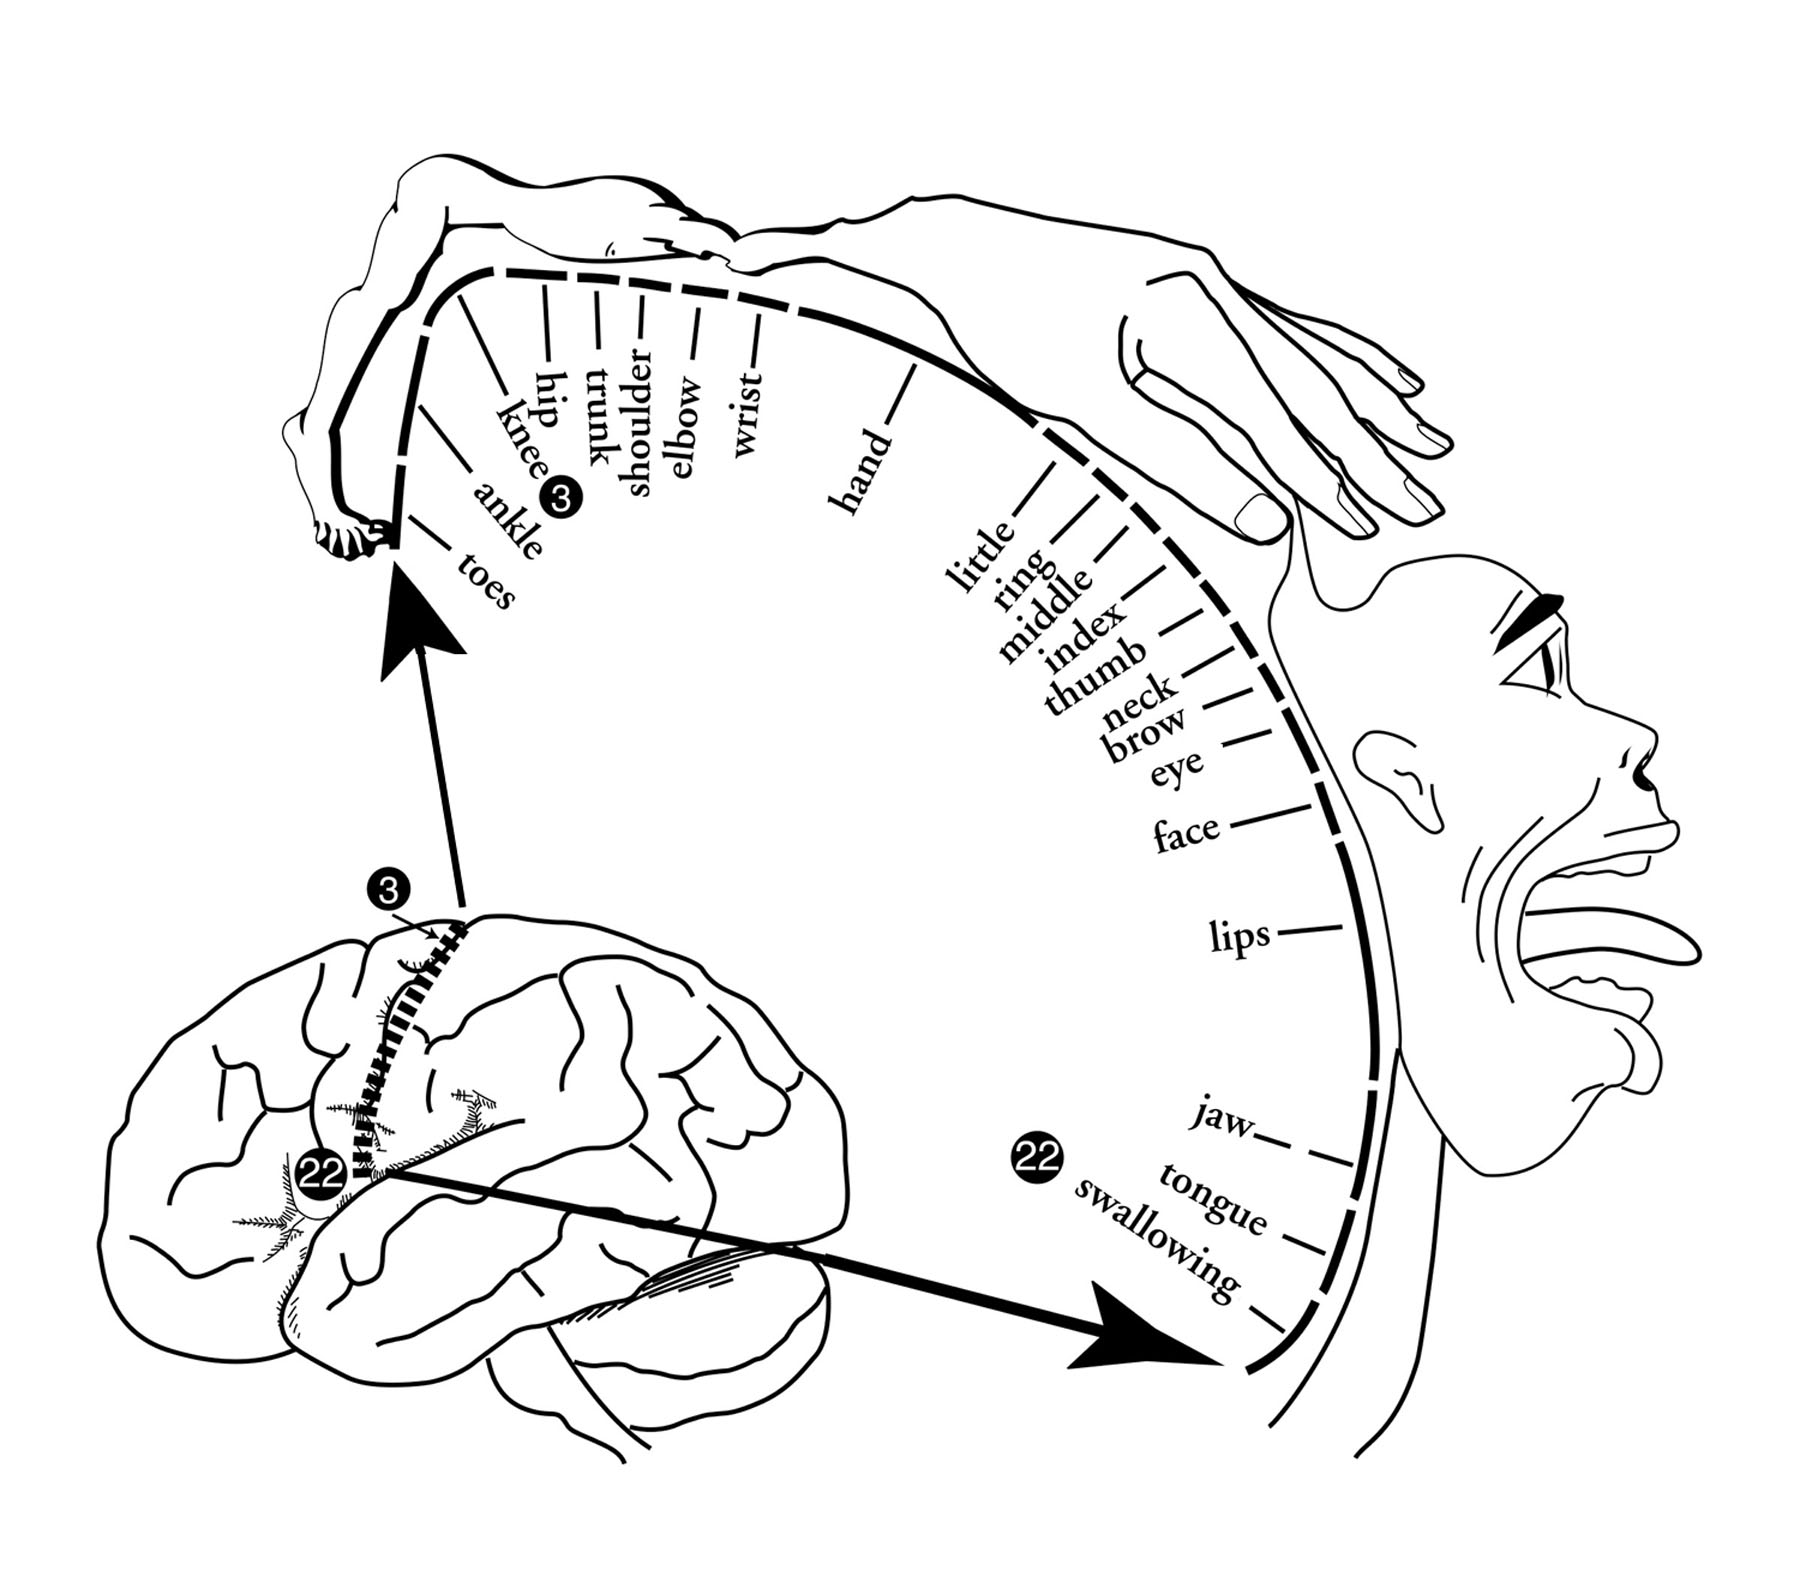
\includegraphics[width=3in]{./kap/bilder/homunc.jpg}}%!!! må byttes ut, copyright Greys anatomy
                      \caption{her ser vi kroppen bredt utover hjernebarken}
                      %{Her ser vi et bilde som illusterer lungene og den antomiske oppbygningen}%\textit{tjenestetilbudene}.]
                    \end{figure}
			\paragraph{Sykdommer i nervescellene\\}
				Demens forårsakes av at det lagres et protein som heter tau(egentlig den greske bokstaven T), og som ødelegger nervecellene det lagres inne i. Det finnes flere typer demens og behandlingen er forskjellig. Mest kjent er Alzheimers demens. I dag er demens en sykdom som ikke har god behandling. Det finnes noen medisiner som reduserer symptomer men det er oftest kortvarig. 
		\section{Klinikk}
			\subsection{Slag og drypp}
				Det varierer litt med hva som står på norsk og hva som var ment på engelsk\cite{!!!}%NEL referanse
				. Særlig er det viktig å huske forkortelsen FAST(Fjeset - Armen - Språk - Tid), de tre første er symptomer den siste skal minne oss på at det haster. I dag kan mange få sterkt bedret forløp av å få rask behandling. Symptomene kommer ofte brått og kan noen ganger føre til at pasienten blir bevisstløs eller kramper. Dette er veldig skremmende å oppleve dersom man er den første som finner pasienten. 
			\subsection{Demens}
				At det finnes forkjellige typer for demens er kjent for mange. Det er viktig å vite fordi behandlingen kan være forskjellig og måten man skla håndtere pasienten er ofte forkjellig. Det kan være enkelte hendelser man skal være forberdt på med bestemte typer demens, mer om det \ref{lewy-body}. Alle demenssykdommer rammer hele familien hardt og de fleste pårørende trenger mye støtte i forløpet av en slik sykdom.
				\subsubsection{Alzheimers}
					Alzheimers er den hyppigte demensformen. Det er bestemte deler av hjernen som forvitrer på grunn av en innlagring av proteiner som kroppen ikke klarer å bryte ned. Sykdommen er dødelig og det finnes ingen behandling. I gjennomsnitt er man syk i 5 -15 år før man dør. I perioden før man dør er det ofte et stort pleiebehov. Noen verktøy som brukes: MMS(Mini mental status - en enkel test av kognitiv funksjon), Trailmaking A og B(To tester for sjekke hvor godt man klarer å følge sammenhenger i tall og bokstaver i et spor over en side- brukes i Demensutredningen) og Klokketesten(Tegn en analog klokke som viser for eksempel 10 på to). 
				\subsubsection{Andre former for demens}
					\paragraph{Lewy- Body demens\\}
						Noen pasienter utvikler en demens med sterkt varierende dagsform og parkinsonaktige bevegelser(skjelving osv). Denne formen kalles Lewy Body som er navnet på artefakter som ses i hjernen på pasientene. På grunn av den sterkt varierende dagsformen kan disse være vanskeligere å få diagnostisert skikkelig.
					\paragraph{Frontallappsdemens\\}
						I frontallappen sitter personligheten vår og denne demenstypen gir også sterke forandringer i personligheten og aggressjon som skiller seg fra Alzheimer demensen.
					\paragraph{Degenerative forandringer; Åreforkalkning\\}
						Denne samlebetegnelsen tas med her selv om den strengt tatt burde holdes adskilt fra de to nevnt over. Det er fordi de skiller seg på måte hjernen ødelegges på. Dette er en diffus dårlig blodsirkulasjon som gjør at hjernen blir ødelagt på grunn av dårlig blodgjennomstrømning. Dette er ofte et funn på CT eller MR som er gjort i en demens utredning.
		\section{Pasienteksempler}
			Disse pasientene er tenkt til diskusjon, det finnes derfor ingen fasit. 
			\subsection{Pasient 3}
				Ella, 56 år gammel enslig kvinne, bosatt i Midt-Norge jobber som kunstner. I det siste er det kommet bekymringsmeldinger til fastlegen, kommunen og politiet fordi hun er aggressiv og virker ustellt og det er rotete omkring huset hennes. Det er ukjent hvor lenge hun har holdt på slikt. Hun har lite sosialt nettverk.\\
					\begin{itemize}
						\item Hva er det som gjør at pasienten trenger bred utredning?\\
						\item Hva gjør en demensdiagnose med samtykkekompetansen?\\
						\item Hvis hun motsetter seg utredning, kan hun tvinges?\\
						\item Hvem bestemmer om pasienten er samtykkekompetent?\\
					\end{itemize}
			\subsection{Pasient 4}
				Olav 76 bor sammen med kona og har tidligere jobbet som snekker. For to år siden fikk han diagnosen Alzheimers demens etter han første gang for tre år siden forsvant fra hjemmet og ble funnet tre dager senere i utenfor barndomshjemmet flere hundre kilometer unna hjemstedet. Nå har kona behov for mer tilrettelegging i hjemmet. Han er også truende i perioder, som gjør at kona blir engstelig. \\
				Nå ligger han i sengen og plukker på tapeten. - Det er små dyr, sier han. - De kravler oppover veggen her og skal stjele motorsykkelen min. Ser du ikke det?\\
				Kona forteller at han de siste to dagene har blitt rar og at han har ramlet noen ganger. Det er derfor hun har ringt på trygghetsalarmen.\\

					\begin{itemize}
						\item Hva slags tilstand er dette?\\
						\item Hvordan begynner man å behandle dette?\\
						\item Hva sier du til kona?\\
						\item Hvor farlig er dette?\\
						\item Er demensen blitt verre på grunn av dette?\\
						\item Kona er bekymret for at hans skal komme hjem igjen. Hva sier du til henne?\\
					\end{itemize}	


\newpage